\documentclass[tikz,border=6pt]{standalone}
% Shared visual language for the original benchmark atlas.
\usepackage[T1]{fontenc}
\usepackage{lmodern}
\usepackage{amsmath,amssymb}
\usetikzlibrary{arrows.meta,calc,positioning,shapes.geometric,patterns,decorations.pathmorphing,backgrounds,fit}
\definecolor{ink}{HTML}{173948}
\definecolor{flow}{HTML}{167D9A}
\definecolor{control}{HTML}{A65217}
\definecolor{measure}{HTML}{70518A}
\definecolor{pale}{HTML}{EAF2F5}
\definecolor{muted}{HTML}{526571}
\definecolor{utility}{HTML}{2E8665}
\tikzset{
  every node/.style={font=\sffamily\small,text=ink},
  equipment/.style={draw=ink,line width=1pt,fill=pale,rounded corners=2pt},
  process/.style={draw=flow,line width=1.2pt,-{Latex[length=2.5mm]}},
  signal/.style={draw=control,line width=.8pt,dashed,-{Latex[length=2mm]}},
  util/.style={draw=utility,line width=1pt,-{Latex[length=2.2mm]}},
  dimension/.style={draw=muted,line width=.6pt,{Latex[length=1.7mm]}-{Latex[length=1.7mm]}},
  labelbox/.style={fill=white,inner sep=2pt,font=\sffamily\footnotesize,align=center},
  annotation/.style={font=\sffamily\footnotesize,text=muted,align=left},
  panel/.style={draw=ink!20,fill=ink!2,rounded corners=3pt,inner sep=6pt},
  instrument/.style={circle,draw=measure,fill=white,line width=.8pt,minimum size=8mm,inner sep=1pt,font=\sffamily\scriptsize,align=center},
  port/.style={circle,fill=flow,inner sep=1.6pt},
  box/.style={equipment,minimum width=3cm,minimum height=1cm,align=center},
}
\newcommand{\atlasheader}[3]{%
  \node[anchor=north west,font=\sffamily\bfseries\LARGE] at (0,0) {#1};%
  \node[anchor=north west,font=\sffamily\small,text=muted] at (0,-.75) {Paper section #2: \textit{#3}};%
  \draw[ink!25,line width=.7pt] (0,-1.25)--(26,-1.25);%
}
\newcommand{\atlasfooter}[1]{%
  \draw[ink!25,line width=.5pt] (0,-15.8)--(26,-15.8);%
  \node[anchor=north west,annotation,text width=25.8cm] at (0,-16) {#1\\Original explanatory drawing. Source: Kroll \& Schulte (2014), DOI: 10.1016/j.asoc.2014.08.034. Model variants are identified in the accompanying case sheet.};%
}

\begin{document}
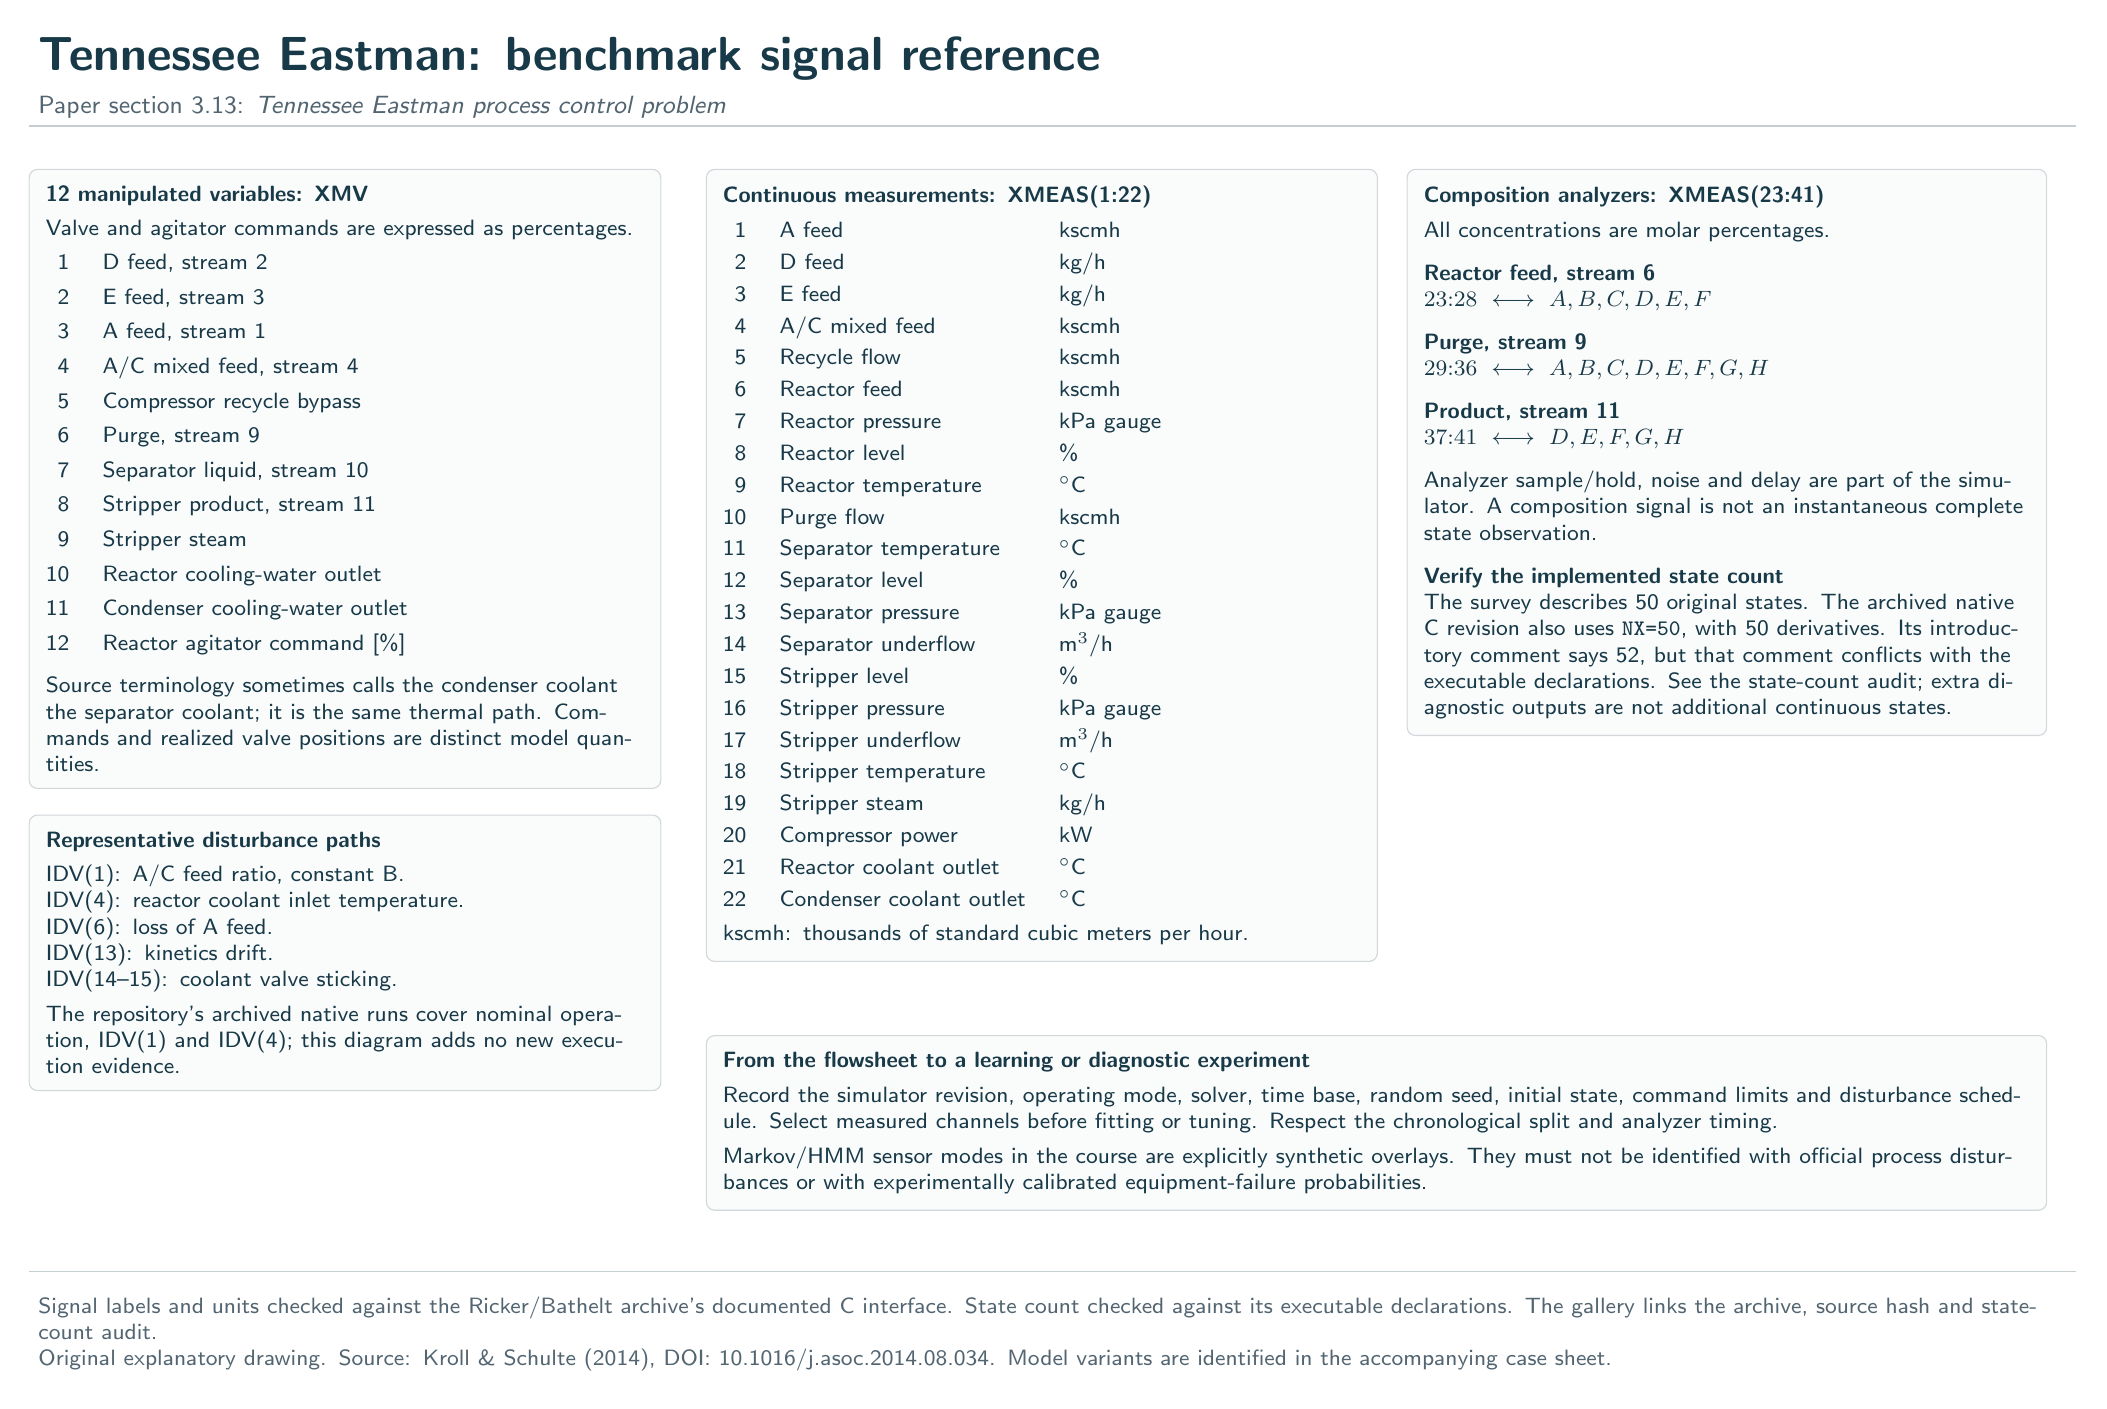
\begin{tikzpicture}[x=1cm,y=1cm]
\atlasheader{Tennessee Eastman: benchmark signal reference}{3.13}{Tennessee Eastman process control problem}
\node[panel,anchor=north west,text width=7.6cm,align=left,font=\sffamily\footnotesize]at(0,-1.8){
\textbf{12 manipulated variables: XMV}\par\smallskip
Valve and agitator commands are expressed as percentages.\par\smallskip
\begin{tabular}{@{}rl@{}}
1 & D feed, stream 2\\[3pt]
2 & E feed, stream 3\\[3pt]
3 & A feed, stream 1\\[3pt]
4 & A/C mixed feed, stream 4\\[3pt]
5 & Compressor recycle bypass\\[3pt]
6 & Purge, stream 9\\[3pt]
7 & Separator liquid, stream 10\\[3pt]
8 & Stripper product, stream 11\\[3pt]
9 & Stripper steam\\[3pt]
10 & Reactor cooling-water outlet\\[3pt]
11 & Condenser cooling-water outlet\\[3pt]
12 & Reactor agitator command [\%]
\end{tabular}\par\medskip
Source terminology sometimes calls the condenser coolant the separator coolant; it is the same thermal path. Commands and realized valve positions are distinct model quantities.};
\node[panel,anchor=north west,text width=8.1cm,align=left,font=\sffamily\footnotesize]at(8.6,-1.8){
\textbf{Continuous measurements: XMEAS(1:22)}\par\smallskip
\begin{tabular}{@{}rll@{}}
1&A feed&kscmh\\[2pt]
2&D feed&kg/h\\[2pt]
3&E feed&kg/h\\[2pt]
4&A/C mixed feed&kscmh\\[2pt]
5&Recycle flow&kscmh\\[2pt]
6&Reactor feed&kscmh\\[2pt]
7&Reactor pressure&kPa gauge\\[2pt]
8&Reactor level&\%\\[2pt]
9&Reactor temperature&$^\circ$C\\[2pt]
10&Purge flow&kscmh\\[2pt]
11&Separator temperature&$^\circ$C\\[2pt]
12&Separator level&\%\\[2pt]
13&Separator pressure&kPa gauge\\[2pt]
14&Separator underflow&m$^3$/h\\[2pt]
15&Stripper level&\%\\[2pt]
16&Stripper pressure&kPa gauge\\[2pt]
17&Stripper underflow&m$^3$/h\\[2pt]
18&Stripper temperature&$^\circ$C\\[2pt]
19&Stripper steam&kg/h\\[2pt]
20&Compressor power&kW\\[2pt]
21&Reactor coolant outlet&$^\circ$C\\[2pt]
22&Condenser coolant outlet&$^\circ$C
\end{tabular}\par\smallskip
kscmh: thousands of standard cubic meters per hour.};
\node[panel,anchor=north west,text width=7.7cm,align=left,font=\sffamily\footnotesize]at(17.5,-1.8){
\textbf{Composition analyzers: XMEAS(23:41)}\par\smallskip
All concentrations are molar percentages.\par\medskip
\textbf{Reactor feed, stream 6}\par
$23{:}28\ \longleftrightarrow\ A,B,C,D,E,F$\par\medskip
\textbf{Purge, stream 9}\par
$29{:}36\ \longleftrightarrow\ A,B,C,D,E,F,G,H$\par\medskip
\textbf{Product, stream 11}\par
$37{:}41\ \longleftrightarrow\ D,E,F,G,H$\par\medskip
Analyzer sample/hold, noise and delay are part of the simulator. A composition signal is not an instantaneous complete state observation.\par\medskip
\textbf{Verify the implemented state count}\par
The survey describes 50 original states. The archived native C revision also uses \texttt{NX=50}, with 50 derivatives. Its introductory comment says 52, but that comment conflicts with the executable declarations. See the state-count audit; extra diagnostic outputs are not additional continuous states.};
\node[panel,anchor=north west,text width=7.6cm,align=left,font=\sffamily\footnotesize]at(0,-10.0){
\textbf{Representative disturbance paths}\par\smallskip
IDV(1): A/C feed ratio, constant B.\par
IDV(4): reactor coolant inlet temperature.\par
IDV(6): loss of A feed.\par
IDV(13): kinetics drift.\par
IDV(14--15): coolant valve sticking.\par\smallskip
The repository's archived native runs cover nominal operation, IDV(1) and IDV(4); this diagram adds no new execution evidence.};
\node[panel,anchor=north west,text width=16.6cm,align=left,font=\sffamily\footnotesize]at(8.6,-12.8){
\textbf{From the flowsheet to a learning or diagnostic experiment}\par\smallskip
Record the simulator revision, operating mode, solver, time base, random seed, initial state, command limits and disturbance schedule. Select measured channels before fitting or tuning. Respect the chronological split and analyzer timing.\par\smallskip
Markov/HMM sensor modes in the course are explicitly synthetic overlays. They must not be identified with official process disturbances or with experimentally calibrated equipment-failure probabilities.};
\atlasfooter{Signal labels and units checked against the Ricker/Bathelt archive's documented C interface. State count checked against its executable declarations. The gallery links the archive, source hash and state-count audit.}
\end{tikzpicture}
\end{document}
